\documentclass{article}
\usepackage[utf8]{inputenc}
\usepackage[T1]{fontenc}
\usepackage[export]{adjustbox}
\usepackage{mathtools,amsthm,amssymb,icomma,upgreek,xfrac,enumerate, bbm,titlesec,lmodern,polski,derivative,geometry,multicol,titling,graphicx,url,amsmath,caption,lipsum,float,longtable,booktabs}
\usepackage[table,xcdraw]{xcolor}
\usepackage[hidelinks,breaklinks,pdfusetitle,pdfdisplaydoctitle]{hyperref}
\usepackage{listings}
\definecolor{codegreen}{rgb}{0,0.6,0}
\definecolor{codegray}{rgb}{0.5,0.5,0.5}
\definecolor{codepurple}{rgb}{0.58,0,0.82}
\definecolor{backcolour}{rgb}{0.95,0.95,0.92}
\definecolor{light-gray}{gray}{0.95}
\setlength{\droptitle}{-1cm}
\mathtoolsset{showonlyrefs,mathic}
\title{Dokumentacja}
\author{Zuzanna Bilińska, Joanna Kołaczek, Łukasz Simbiga, Filip Lasko}
\date{\today}
\newtheoremstyle{break}
{\topsep}{\topsep}%
{\normalfont}{}%
{\bfseries}{}%
{\newline}{}%
\theoremstyle{break}

\titleformat*{\section}{\LARGE\bfseries}
\titleformat*{\subsection}{\Large\bfseries}
\titleformat*{\subsubsection}{\large\bfseries}
\titleformat*{\paragraph}{\large\bfseries}
\titleformat*{\subparagraph}{\large\bfseries}

\lstdefinestyle{mystyle}{
	backgroundcolor=\color{backcolour},   
	commentstyle=\color{codegreen},
	keywordstyle=\color{magenta},
	numberstyle=\tiny\color{codegray},
	stringstyle=\color{codepurple},
	basicstyle=\ttfamily\footnotesize,
	breakatwhitespace=false,         
	breaklines=true,                 
	captionpos=b,                    
	keepspaces=true,                 
	numbers=left,                    
	numbersep=5pt,                  
	showspaces=false,                
	showstringspaces=false,
	showtabs=false,                  
	tabsize=2
}

\lstset{style=mystyle}
\renewcommand{\lstlistingname}{Kod}% Listing -> Kod
\renewcommand{\lstlistlistingname}{Lista Kodów}% List of Listings -> Lista kodów
\newcommand{\code}[1]{\colorbox{light-gray}{\texttt{#1}}}


\begin{document}
	\maketitle
	\tableofcontents
	\clearpage
	
	
	\section{Wstęp}
	W dokumencie tym przedstawiono najważniejsze informację dotyczące projektu: Bazy danych. 
	Zespół, będący autorem projektu, pracował w składzie: Zuzanna Bilińska, Joanna Kołaczek, Łukasz Simbiga, Filip Lasko. Tematy, które opracowaliśmy to:
	\begin{itemize}
		\item utworzenie schematu,
		\item wypełnianie bazy,
		\item analiza danych,
		\item raport,
		\item dokumentacja.
	\end{itemize}
	
	\section{Spis użytych technologii}
	Technologie użyte podczas projektu Bazy danych:
	\begin{itemize}
		\item MariaDB,
		\item Python - użyte biblioteki: mysql.connector, pandas, random, math, numpy, datetime, matplotlib.pyplot, plotly, io,
		\item Python - Jupyter Notebook,
		\item TeX - TeXstudio.
	\end{itemize}
	\section{Lista Plików}
	Lista plików, które utworzyliśmy podczas projektowania bazy danych:
	\begin{itemize}
		\item Generowanie\_danych.ipynb,
		\item Sposób\_generowania\_danych.pdf,
		\item Raport\_BD.ipynb,
		\item Dokumentacja.pdf,
		\item html\_report.html.
	\end{itemize}
	\section{Kolejność i sposób uruchamiania plików}
	\paragraph{Utworzenie bazy danych}
	Zanim otworzysz plik sql\_in\_python.ipynb pamiętaj, że baza danych została już utworzona na serwerze giniewicz.it, więc zbędne jest uruchamianie tych plików i~ponowne tworzenie bazy danych, jednak jeżeli naszym celem jest jej kreacja, powinniśmy uruchomić plik sql\_in\_python.ipynb. Otworzyć możemy go tylko i wyłącznie za pomocą Jupyter Notebook. W notatniku za pomocą funkcji create\_db\_connection($\dots$) łączymy się z bazą danych, a następnie za pomocą odpowiednich funkcji tworzymy tabele oraz je wypełniamy. Kontekst ten został szerzej opisany w dokumencie Sposób\_generowania\_danych.pdf. \\
	\paragraph{Analiza oraz raport}
	Zanim otworzysz plik Raport\_BD.ipynb, raport możesz zobaczyć w~pliku html\_report.html. Jeżeli natomiast nie posiadamy tego dokumentu, powinniśmy go utworzyć. Uruchamiamy wtedy plik Raport\_BD.ipynb w Jupyter Notebook, aby następnie połączyć się z bazą danych za pomocą funkcji create\_db\_connection($\dots$). Następnie, po wywołaniu reszty funkcji, w~szczególności:
	$$\begin{multlined}
			with \ open('html\_report.html'\ ,\ 'w') \ as \  f: \\
			f.write(html),
	\end{multlined}$$
	powstanie nam dokument html\_report.html, przedstawiający raport z zawartą w nim analizą. 
	\paragraph{Dokumentacja}
	Jeżeli chcemy poznać dodatkowe informację o projekcie Bazy danych, powinniśmy uruchomić plik Dokumentacja.pdf.
	
	\section{Schemat projektu bazy danych}
	Na rysunku \ref{fig:schemat} przedstawiony został schemat bazy danych, łącznie wyprodukowaliśmy siedem tabel, z czego każda tabela zawiera, co najmniej 3 kolumny z danymi. Baza danych przechowuje informację o:
	\begin{itemize}
		\item klientach,
		\item pracownikach,
		\item sprzedaży gier,
		\item wypożyczeniu gier,
		\item odbytych turniejach,
		\item asortymencie,
		\item wynikach turniejów.
	\end{itemize}


	\begin{figure}[H]
		\begin{center}
			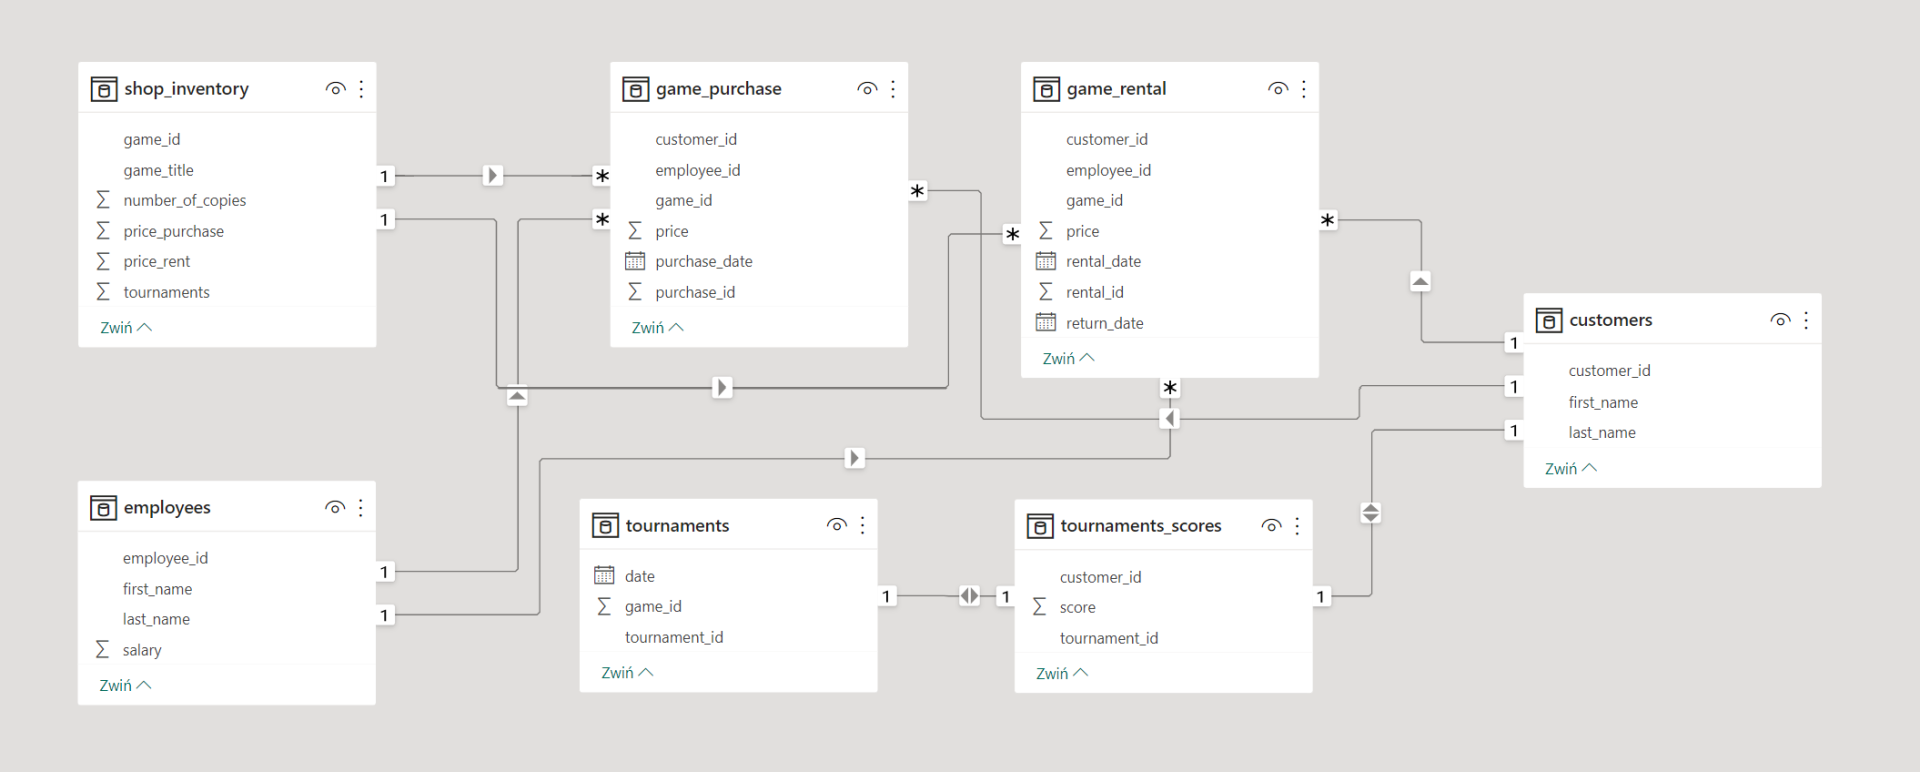
\includegraphics[scale=0.22]{schemat.png}
			\caption{Schemat bazy danych}
			\label{fig:schemat}
		\end{center}
	\end{figure}
	
	\section{Lista zależności funkcyjnych}

	\hspace{0.5cm}Zależność funkcyjna to pojęcie używane w kontekście baz danych relacyjnych, które opisuje zależność między atrybutami w tabeli. Mówiąc prościej, zależność funkcyjna oznacza, że wartość jednego lub więcej atrybutów w tabeli jednoznacznie determinuje wartość innego atrybutu. Reprezentowana jest w postaci $A \rightarrow B$, gdzie A i B są zbiorami atrybutów. Oznacza to, że dla każdej kombinacji wartości atrybutów w zbiorze A, istnieje jednoznacznie określona wartość atrybutu lub atrybutów w~zbiorze B. Może to oznaczać, że jeden atrybut determinuje inny, lub że grupa atrybutów determinuje inną grupę atrybutów.
	
	W rozdziale tym zostaną zaprezentowane zależności funkcyjne, wystepujące w bazie danych, której schemat został zaprezentowany na rysunku \ref{fig:schemat}. Dla każdej tabeli opiszemy występujące atrybuty oraz znajdziemy zależności funkcyjne, aby określić możliwe nadklucze, z których poźniej wybierzemy klucz główny.
	
	\paragraph{Customers}
	\begin{table}[!ht]
		\centering
		\begin{tabular}{|c|c|c|}
			\hline
			customer\_id & first\_name & last\_name \\ \hline
			1 & Łukasz & Simbiga\\ \hline
			2 & Wiktoria & Simbiga \\ \hline
			\vdots & \vdots & \vdots \\ \hline
			1850 & Piotr & Krawczyk \\ \hline
		\end{tabular}
		\caption{Customers.}
		\label{table:customers}
	\end{table}
	W tabeli \ref{table:customers} przedstawiono część danych o klientach wraz z przypisanymi im atrybutami:
	\begin{itemize}
		\item $customer\_id_{INT}$ - numer klienta, przypisywany inny dla każdego klienta,
		\item $first\_name_{STR}$ - imię klienta,
		\item $last\_name_{STR}$ - nazwisko klienta.
	\end{itemize}
	Relacja jaką tworzy ta tabela zapisana może zostać następująco:
	$$ Customers=\{(1, Lukasz, Simbiga), \dots,(1850, Piotr, Krawczyk)\}.  $$
	Z powyższych atrybutów jedynie \{customer\_id\} jest unikatowe, ponieważ tylko w kolumnie, opisanej tym atrybutem, nie występują powtórzenia. Dodatkowo, połączenie atrybutów \{first\_name, last\_name\} nie gwarantuje nam unikatowości, ponieważ w bazie klientów występują osoby o takim samym imieniu i nazwisku. Stąd posiadać będziemy 4 nadklucze: \{customer\_id\}, \{customer\_id, first\_name\}, \{customer\_id, last\_name\}, \{customer\_id, first\_name, last\_name\}. Z czego tylko \{customer\_id\} spełnia definicje klucza kandydującego, więc jest kluczem głównym. 
	
	Zależności funkcyjne, występujące w tabeli Customers, opisać możemy następująco:
	$$ \Sigma = \{ A \rightarrow ABC \}, \\ $$
	gdzie: 
	\begin{itemize}
		\item A to customer\_id,
		\item B to first\_name,
		\item C to last\_name.
	\end{itemize}
	Tak jak wspominaliśmy jedynie atrybut/zbiór atrybutów: \{customer\_id\} jest unikatowy. Tylko znajomość numeru klienta gwarantuje nam możliwość poznania wszystkich innych danych tego samego klienta z tabeli \ref{table:customers}, dlatego też zastosowana powyżej zależność funkcyjna jest dobrze opisana.	
	
	
	\paragraph{Employees}
	
	\begin{table}[!ht]
		\centering
		\begin{tabular}{|c|c|c|c|}
			\hline
			employee\_id & first\_name & last\_name & salary \\ \hline
			1 & Adam & Plotnik & 4200\\ \hline
			2 & Błażej & Słowik & 4500 \\ \hline
			\vdots & \vdots & \vdots & \vdots \\ \hline
			8 & Damian & Skóra & 4400 \\ \hline
		\end{tabular}
		\caption{Employees.}
		\label{table:employees}
	\end{table}
	W tabeli \ref{table:employees} zoabczyć możemy część danych o pracownikach oraz przypisane im~atrybuty:
	\begin{itemize}
		\item $employee\_id_{INT}$ - numer pracownika, przypisywany inny dla każdego pracownika,
		\item $first\_name_{STR}$ - imię pracownika,
		\item $last\_name_{STR}$ - nazwisko pracownika,
		\item $salary_{INT}$ - zarobki pracownika.
	\end{itemize}
	Relacja jaką tworzy nam ta tabela zostać może zapisana następująco:
	$$ Employees=\{(1, Adam, Plotnik, 4200), \dots,(8, Damian, Skora, 4400)\}. $$
	Z powyższej relacji moglibyśmy wypisać wiele występujących nadkluczy. Jednak wśród nich występują 3 klucze kandydujące, które zarazem są atrybutami głównymi: \{employee\_id\}, \{first\_name\}, \{last\_name\}. Jest tak, ponieważ każdy z tych atrybutów jest unikatowy dla tabeli \ref{table:employees}. Następnie możemy wybrać klucz główny, którym będzie \{employee\_id\}. 	
	Zależności funkcyjne, występujące w~tabeli Employees, opisać możemy następująco:
	$$ \Sigma = \{ A \rightarrow ABCD, B\rightarrow ABCD, C\rightarrow ABCD \}, \\ $$
	gdzie: 
	\begin{itemize}
		\item A to employee\_id,
		\item B to first\_name,
		\item C to last\_name,
		\item D to salary.
	\end{itemize}
	Powodem  wyboru takich zależności funkcyjnych był fakt, że każdy z atrybutów A,B,C jest unikatowy, jednak liczyć się trzeba z uwagą, iż przybycie do grona pracowników osoby o identycznym imieniu bądź nazwisku, skutkować będzie usunięciem odpowiedniej pozycji z~grona zależności funkcyjnych. Przykładem może być pojawienie się pracownika o takim samym imieniu jak jeden z~aktualnych pracowników,lecz różnych zarobkach, wtedy zależności funkcyjne opiszemy:  
	$$ \Sigma = \{ A \rightarrow ABCD, C\rightarrow ABCD, BD\rightarrow ABCD  \}. \\ $$
	
	
	
	
	
	\paragraph{Game\_purchase}
	\begin{table}[!ht]
		\centering
		\begin{tabular}{|c|c|c|c|c|c|}
			\hline
			purchase\_id & customer\_id & game\_id & employee\_id & purchase\_date & price \\ \hline
			1 & 1 & 4 & 3 & 2020-04-22 & 100.00\\ \hline
			2 & 2 & 65 & 1 & 2020-04-22 & 60.00\\ \hline
			\vdots & \vdots & \vdots & \vdots & \vdots & \vdots \\ \hline
			5807 & 1850 & 44 & 7 & 2022-02-14 & 125.00 \\ \hline
		\end{tabular}
		\caption{Game\_purchase.}
		\label{table:game_purchase}
	\end{table}
	W tabeli \ref{table:game_purchase} przedstawiono część danych, które odpowiadają za informację o~sprzedanych grach. Dodatkowo, w tabeli znajdziemy atrybuty reprezentujące odpowiednie kolumny:
	\begin{itemize}
		\item $purchase\_id_{INT}$ - numer sprzedaży,
		\item $customer\_id_{INT}$ - numer klienta, który zakupił grę,
		\item $game\_id_{INT}$ - numer inforumujący, jaka gra została sprzedana,
		\item $employee\_id_{INT}$ - numer pracownika, który sprzedał grę,
		\item $purchase\_date_{DATE}$ - data sprzedaży,
		\item $price_{DECIMAL}$ - cena, po której sprzedano grę.
	\end{itemize}
	Relacje zawartą w tabeli \ref{table:game_purchase} opisać możemy następująco:
	$$ Game\_purchase=\{(1, 1, 4, 3,2020\--04\--22,100.00), \dots,(	5807, 1850, 44, 7, 2022\--02\--14, 125.00)\}.  $$
	Dla powyższej relacji, wybranie \{purchase\_id\} jako klucza głównego jest jedynym sensownym pomysłem. Zapewnia nam on występowanie, co najmnej jednej zależności funkcyjnej:
	$$ \Sigma = \{A \rightarrow ABCDEF , BCE\rightarrow ABCDEF  \}, \\ $$
	gdzie:
		\begin{itemize}
		\item A to purchase\_id,
		\item B to customer\_id,
		\item C to game\_id,
		\item D to employee\_id,
		\item E to purchase\_date,
		\item F to price.
	\end{itemize}
	Z przyczyn oczywistych pojawia się w gronie zależności funkcyjnych: $A \rightarrow ABCDEF$. Co ciekawe, do tego grona dołączyć możemy dołączyć $BCE\rightarrow ABCDEF$, ponieważ klucz kandydujący \{customer\_id, game\_id, purchase\_date\} jest unikatowy. Wpisując dowolne dane pod te atrybuty, jesteśmy w stanie poznać resztę informacji o odnotowanej sprzedaży. 
	
	
	\paragraph{Game\_rental}
	
	
	\begin{table}[!ht]
		\centering
		\begin{tabular}{|c|c|c|c|c|c|c|}
			\hline
			rental\_id & customer\_id & game\_id & employee\_id & rental\_date & return\_date & price \\ \hline
			1 & 1 & 43 & 2 & 2020-04-21 & 2020-05-18 & 30.00\\ \hline
			2 & 2 & 65 & 1 & 2020-04-22 & 2020-05-18 & 15.00\\ \hline
			\vdots & \vdots & \vdots & \vdots & \vdots & \vdots & \vdots \\ \hline
			19397 & 1850 & 58 & 3 & 2022-02-14 & NULL & 30.00 \\ \hline
		\end{tabular}
		\caption{Game\_rental.}
		\label{table:game_rental}
	\end{table}
	W tabeli \ref{table:game_rental} przedstawiono część danych, które odpowiadają za informację o~wypożyczonych grach. Dodatkowo, w tabeli znajdziemy atrybuty reprezentujące odpowiednie kolumny:
	\begin{itemize}
		\item $rental\_id_{INT}$ - numer wypożyczenia,
		\item $customer\_id_{INT}$ - numer klienta, który wypożyczył grę,
		\item $game\_id_{INT}$ - numer inforumujący, jaka gra została wypożyczona,
		\item $employee\_id_{INT}$ - numer pracownika, który wypożyczył grę,
		\item $rental\_date_{DATE}$ - data wypożyczenia gry,
		\item $return\_date_{DATE}$ - data zwrotu gry,
		\item $price_{DECIMAL}$ - cena, po której sprzedano grę.
	\end{itemize}
	Relacje zawartą w tabeli \ref{table:game_rental} opisać możemy następująco:
	$$
	\begin{multlined}
	Game\_rental=\{(1, 1, 43, 2,2020-04-21,2020-05-18,30.00), \dots,\\
	 (19397, 1850, 58, 3, 2022\--02\--14,NULL, 30.00)\}. 	
	\end{multlined}
	$$  
	Jako klucz główny najlepiej w tym wypadku przyjąć \{rental\_id\}. Atrybut ten jest unikatowy dla każdej pozycji w danych. Tak, jak w przypadku Game\_purchase zapewnieni jesteśmy o tym,~że~atrybut główny utworzy nam zależność funkcyjna z każdym innym atrybutem, jednak sprawdźmy, czy istnieją jakieś inne zależności: 
	$$ \Sigma = \{A \rightarrow ABCDEFG \}, \\ $$
	gdzie:
	\begin{itemize}
		\item A to rental\_id,
		\item B to customer\_id,
		\item C to game\_id,
		\item D to employee\_id,
		\item E to rental\_date,
		\item F to return\_date,
		\item G to price.
	\end{itemize}
	Niestety nie doszukaliśmy się innych zależności funkcyjnych w tabeli \ref{table:game_rental}. Powodem tej sytuacji jest najprawdopodobniej fakt, iż nasza tabela posiada, aż 19397 wierszy. Gdybyśmy nie uwzględnili atrybutu \{rental\_id\}, to w tabeli występowały duplikaty. Chociażby wywołanie danych BCDEFG, nie gwarantuje nam, że poznamy informację kryjącą sie pod A, ponieważ w naszej wypożyczalni wystąpiła sytuacja, że ten sam klient wypożyczył 2 razy tę samą grę, tego same dnia i tę 2 gry zwrócił w tym samym dniu. Obsługiwał go ten sam pracownik i zapłacił taką samą cenę. Dodatkowo, nie znaleźliśmy powiązań między poszczególnymi atrybutami, więc zakończyliśmy poszukiwania zależności funkcyjnych.

	\paragraph{Game\_tournaments}
	\begin{table}[!ht]
		\centering
		\begin{tabular}{|c|c|c|}
			\hline
			tournament\_id & tournament\_date & game\_id \\ \hline
			1 & 2020-06-06 17:00 & 1 \\ \hline
			2 & 2020-07-04 16:00 & 2 \\ \hline
			\vdots & \vdots & \vdots  \\ \hline
			25 & 2022-06-03 10:00 & 1 \\ \hline
		\end{tabular}
		\caption{Game\_tournaments.}
		\label{table:game_tournaments}
	\end{table}
	W tabeli \ref{table:game_tournaments} zaprezentowano część danych inforumjących o odbytych turniejach oraz przypisane im atrybuty:
	\begin{itemize}
		\item $tournament\_id_{INT}$ - numer turnieju, przypisywany inny dla każdego turnieju,
		\item $tournament\_date_{DATETIME}$ - data odbycia turnieju,
		\item $game\_id_{INT}$ - numer gry.
	\end{itemize}
	Relacja jaka tworzy nam tabela \ref{table:game_tournaments}, możemy zapisać następująco:
	$$Game\_tournaments=\{(1,2020-06-06 \ 17:00, 1),\dots,(25,2020-06-03 \ 10:00, 1)\}.$$
	Z powyższej relacji wyłonić możemy dwa atrybuty główne(klucze kandydujące): \{tournament\_id\}, \{tournament\_date\}. Obydwa argumenty pasują do definicji klucza głównego, ponieważ są one unikatowe. Poznając informację ukrytą pod wybranym atrybutem, jesteśmy w stanie odszyfrować resztę danych z tabeli. Kluczem głównym w tej sytuacji zostanie \{tournament\_id\}, ponieważ mamy pewność, że ten atrybut pozostanie unikatowy na zawsze, jeżeli nie zmienimy reguły numeracji turniejów. Z zaistniałych faktów, wyprowadzimy zależności funkcjonalne:
	$$ \Sigma = \{A \rightarrow ABC, B \rightarrow ABC\}, \\ $$
	gdzie:
	\begin{itemize}
		\item A to tournament\_id,
		\item B to tournament\_date,
		\item C to game\_id.
	\end{itemize}
	\paragraph{Shop\_inventory}
	\begin{table}[!ht]
		\centering
		\begin{tabular}{|c|c|c|c|c|c|}
			\hline
			game\_id & game\_title & tournaments & number\_of\_copies & price\_purchase & price\_rent \\ \hline
			1 & Szachy & 1 & 10 & 80 & 20 \\ \hline
			2 & Pandemic Legacy & 1 & 20 & 80 & 20 \\ \hline
			\vdots & \vdots & \vdots & \vdots & \vdots & \vdots  \\ \hline
			81 & Dungeon Lords & 0 & 20 & 60 & 15 \\ \hline
		\end{tabular}
		\caption{Shop\_inventory.}
		\label{table:shop_inventory}
	\end{table}
	W tabeli \ref{table:shop_inventory} przedstawiono część danych, które odpowiadają za informację o grach zanjdujących się w asortymencie. Dodatkowo, w tabeli znajdziemy atrybuty reprezętujące odpowiednie kolumny:
	\begin{itemize}
		\item $game\_id_{INT}$ - numer gry,
		\item $game\_title_{STR}$ - tytuł gry,
		\item $tournaments_{INT}$ - liczba informująca, czy gra jest turniejowa(jeżeli 1 to turniejowa, jeżeli 0 to nie),
		\item $number\_of\_copies_{INT}$ - liczba kopii gier,
		\item $price\_purchase_{INT}$ - cena zakupu gry,
		\item $price\_rent_{INT}$ - cena wypożyczenia gry.
	\end{itemize}
	Relacja, którą tworzy nam tabela \ref{table:shop_inventory} możemy zapisać:
	$$Shop\_inventory = \{(1,Szachy,1,10,80,20),\dots , (81,Dungeon Lordes, 0 ,20,60,15)\}.$$
	Dla powyższej relacji atrybutami głównymi(także kluczami kandydującymi) są: \{game\_id\} oraz \{game\_title\}. Podane atrybuty są unikatowe, dlatego przypisać możemy je do klucza głównego. Tak jak w poprzednich przypadkach, jako klucz główny wybierzemy tylko jeden atrybut, którym będzie \{game\_id\}. Zależności funkcjonalne występujące w tabeli możemy opisać następująco:
	$$ \Sigma = \{A \rightarrow ABCDEF, B \rightarrow ABCDEF\}, \\ $$
	gdzie:
	\begin{itemize}
		\item A to game\_id,
		\item B to game\_title,
		\item C to tournaments,
		\item D to number\_of\_copies,
		\item E to price\_purchase,
		\item F to price\_rent.
	\end{itemize}
	Niestety, żaden z pozostałych argumentów \{C,D,E,F\} oraz kombinacji argumentów, np.: CDEF nie spełnia własności zależności funkcjonalnych. Pomijając atrybuty: \{game\_id\} oraz \{game\_title\} sprawimy, iż w tabeli pojawią się duplikaty.
		
		
	\paragraph{Tournaments\_scores}
	\begin{table}[!ht]
		\centering
		\begin{tabular}{|c|c|c|}
			\hline
			tournament\_id  & customer\_id & score \\ \hline
			1  & 9 & 1  \\ \hline
			1  & 10 & 1  \\ \hline
			\vdots  & \vdots & \vdots   \\ \hline
			21 & 508 & 1  \\ \hline
		\end{tabular}
		\caption{Tournaments\_scores.}
		\label{table:tournaments_scores}
	\end{table}
	W tabeli \ref{table:tournaments_scores} przedstawiono część danych, które odpowiadają za informację o punktach rozdanych konkretnym zawodnikom za konkretne trunieje. Dodatkowo, w tabeli znajdziemy atrybuty reprezentujące odpowiednie kolumny:
	\begin{itemize}
		\item $tournament\_id_{INT}$ - numer turnieju, za który przyznawane są punkty,
		\item $customer\_id_{INT}$ - numer klienta,
		\item $score_{INT}$ - otrzymane punkty.
	\end{itemize}
	Relacja utworzona przez tabele \ref{table:tournaments_scores} opisana może zostać następująco:
	$$Tournaments\_score = \{(1,1,1,10), \dots, (21,201,508,1)\}$$
	Z powyższej relacji wyłonić możemy klucz kandydujący: \{tournament\_id, customer\_id\}, który będzie również kluczem głównym. W tabeli \ref{table:tournaments_scores} nie pojawia się atrybut, który odpowiadałby za numeracja każdego wiersza z osobna, lecz jego role zastępuje kombinacja atrybutów \{tournament\_id, customer\_id\}. Nie jest możliwe, aby ten sam klient wystartował 2 razy w tym samym turnieju, dlatego ta kombinacja jest unikatowa.
	Stąd zależność funkcyjna dla relacji Tournaments\_score wygląda następująco:
		$$ \Sigma = \{A \rightarrow ABC\}, \\ $$
	gdzie:
	\begin{itemize}
		\item A to tournament\_id,
		\item B to customer\_id,
		\item C to score.
	\end{itemize}
	\section{Uzasadnienie, że baza jest w EKNF}
	Relacja jest w postaci normalnej klucza elementarnego (EKNF), jeśli każda nietrywialna zależność funkcyjna albo zaczyna się od nadklucza albo kończy się na atrybucie elementarnym. Definicja ta pozwoli odpowiedzieć nam na pytanie, czy baza danych skonstruowana przez nas jest w EKNF. Zauważyć należy, iż wszystkie zależności funkcyjne opisane przez nas w poprzednim rozdziale, posiadają jedną wspólną cechę: każda zależność funkcyjna zaczyna się od nadklucza. Niemożliwe jest znalezienie atrybutu/kombinacji atrybutów, które nie są nadkluczem, a z których jednoznacznie wynikałoby, że poznanie każdej danej pod tym atrybutem/kombinacją atrybutów pozwoli znaleźć każdą daną ukryta pod innym atrybutem. W skrócie, jeżeli jakiś atrybut/kombinacja atrybutów objaśniały nam inny atrybut, to były to tylko sytuacje, gdy ten atrybut objaśniający był nadkluczem. I taka zależność definiuje naszą bazę danych. Podsumowujac baza danych, skonstruowana przez nas zaespół, jest w postaci normalnej klucza elementarnego (EKNF).
	\section{Napotkane trudności}
	Podczas projektu napotkaliśmy wiele trudności, które opisaliśmy w poniższych punktach:
	\begin{itemize}
	 \item synchornizacja danych - podczas wypełniania tabel dodatkową uwagę musieliśmy poświęcić na zgodność danych pomiędzy tabelami,
	 \item konflikt oznaczeń - różnice w określaniu wartości niezidentyfikowanej(Python - None, MariaDB - NULL) dodały troche trudności podczas wypełniania bazy,
	 \item różnica w indeksowaniu - Python z zasady indeksuje dane w listach/tabelach od 0, my nasze wiersze w tabelach indeksowaliśmy od 1, różnica ta sprawiła nam lekkie problemy podczas analizy danych.
 	\end{itemize}
\end{document}
